\section{Methodology}\label{sec:design}
\renewcommand{\imgpath}{tex/design/imgs}
\vspace{1cm}

\subsection{Overview}
Figure \ref{fig:overview} shows the key steps of the overall method used to go from an image of a lobster to a labelled graph of the lobster. In the initial stages, keypoints are extracted and filtered from the image through the use of various OpenCV algorithms and techniques such as SIFT for keypoint detection and colour histograms for keypoint filtering. The remaining set of keypoints are then labelled using a probabilistic model and all permutations of possible subgraphs are created. 
\begin{figure}[H]
\centering
\begin{subfigure}{\textwidth}
\centering
\begin{tikzpicture}
\node (raw) [data] {Lobster image};
\node (detection) [process, right of=raw, xshift=2cm] {Keypoint detection};
\node (filter) [process, right of=detection, xshift=2cm] {Keypoint filtering};
\node (creation) [process, right of=filter, xshift=2cm] {Subgraph creation};
\node (subgraph) [data, right of=creation, xshift=2cm] {Lobster subgraphs};

\draw [arrow] (raw) -- (detection);
\draw [arrow] (detection) -- (filter);
\draw [arrow] (filter) -- (creation);
\draw [arrow] (creation) -- (subgraph);

\end{tikzpicture}
\caption{Initial process of creating labelled subgraphs for matching.}
\vspace{0.7cm}
\end{subfigure}

\begin{subfigure}{\textwidth}
\centering
\begin{tikzpicture}
\node (subgraph) [data] {Lobster subgraphs};
\node (graphgrep) [process, right of=subgraph, xshift=2cm] {Subgraph matching};
\node (model) [process, right of=graphgrep, xshift=2cm] {Graph building};
\node (graph) [data, right of=model, xshift=2cm] {Matched lobster graph};

\draw [arrow] (subgraph) -- (graphgrep);
\draw [arrow] (graphgrep) -- (model);
\draw [arrow] (model) -- (graph);
\end{tikzpicture}
\caption{Process of taking the labelled subgraphs to creating a full lobster graph.}
\end{subfigure}
\caption{Flow chart of the whole matching process from getting keypoints to creation of the lobster graphs. The yellow steps in the pipeline represent processes and red steps represent inputs and outputs.}
\label{fig:overview}
\end{figure}
\noindent
The second stage of taking a large set of subgraphs and matching them to rebuild the complete lobster graph consists of the following two main steps:
\begin{enumerate}
\item Run GraphGrep to find all subgraphs of valid configurations against the database of complete lobster graphs. 
\item Use the probability of each remaining subgraph to piece together the complete lobster graph.
\end{enumerate}
Finally, to make this all work, a subset of the dataset was taken to create a database of manually annotated attributed lobster graphs. This dataset is important for many aspects of the overall method as it is the set of complete graphs for subgraph matching. Further, the attributes such as node labels, node sizes and edge weights contribute as a basis for the probability models used in both subgraph creation and rebuilding a complete lobster graph. 


\subsection{Annotation of dataset}
The dataset provided by \cite{lobster-thesis} was tagged with information on each image such as the lobster's sex, length of the carapace and width of the tail. To be able to apply the probability models to the dataset and match to complete lobster graphs, the dataset had to be further annotated as attributed graphs. This was initially done and prototyped using Gephi to explore different graph configurations, but only with dummy values for the edge weights and size of the nodes. Later, with the introduction of applying OpenCV keypoint detection algorithms, the annotations were amended with the detected keypoints to include the real node sizes and edge lengths.

\begin{figure}[H]
\centering
\begin{subfigure}{0.31\textwidth}

\end{subfigure}

\begin{subfigure}{0.31\textwidth}

\end{subfigure}

\begin{subfigure}{0.31\textwidth}

\end{subfigure}

TODO Gephi prototype lobster graph
\caption{Examples of different configurations of lobster graphs that were explored on the same lobster image.}
\end{figure}
\noindent
In the initial lobster graph prototyping done with Gephi, different configurations were explored to see how more or less information from the lobster graphs could influence the matching process. At this stage, the use of OpenCV keypoint detectors were not yet used, as the goal was to prototype the graphs and probability models for matching. 
\n
After the use of computer vision algorithms was explored, the annotated step was revisited to update the graphs to correspond to keypoints that could be detected in the images. This improved the annotated dataset by adding more data such as size of nodes and lengths of edges which would be used. This annotation took a few steps to complete:
\begin{enumerate}
\item Run SIFT to detect all keypoints on the image, then output all the keypoints as nodes in \texttt{.gdf} format.
\item By looking at the corresponding images, manually annotate the edge connections between relevant keypoints and remove all other keypoints.
\item Translate the annotated graphs in \texttt{.gdf} format to \texttt{.gfu} format for graph matching tools to use. The \texttt{.gdf} graph formats are still kept as they are used for the probabilistic models.
\end{enumerate}

\imagefig{1\textwidth}{\imgpath/annotated.JPG}{Example of annotated lobster image with nodes and edges of the graph perfectly labelled.}
\noindent
Because the process of manual annotation could have human errors, the final completed annotations are drawn as nodes and edges on top of the raw image again to visually check for mistakes made during the annotation of edges and removal of other keypoints.


\subsection{Keypoint detection}
First, to identify important parts from our lobster images, keypoints or areas of interest must be identified. OpenCV provides a host of different algorithms for feature detection such as Harris and Shi-Tomasi corner detectors and SIFT, SURF, ORB keypoint detectors \cite{opencv-tut1}. All these algorithms were tried and tested on a small subset of the dataset to see if any would provide both useful and consistent features that can be used. 

\begin{figure}[H]
%\centering
	\begin{subfigure}{0.45\textwidth}
	\includegraphics[width=\linewidth, keepaspectratio]{\imgpath/img-harris.png}
	\caption{Harris corner detection}
	\end{subfigure}
	\hspace*{\fill}
	\begin{subfigure}{0.45\textwidth}
	\includegraphics[width=\linewidth, keepaspectratio]{\imgpath/img-shi-tomasi.png}
	\caption{Shi-Tomasi corner detection}
	\end{subfigure}
	
	\vspace{0.5cm}
	
	\begin{subfigure}{0.45\textwidth}
	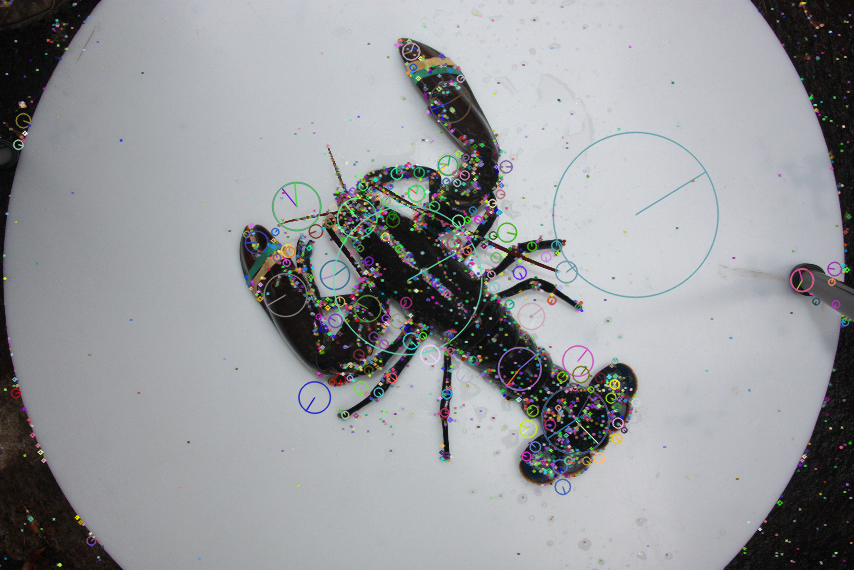
\includegraphics[width=\linewidth, keepaspectratio]{\imgpath/img-sift.png}
	\caption{SIFT keypoint detection}
	\end{subfigure}
	\hspace*{\fill}
	\begin{subfigure}{0.45\textwidth}
	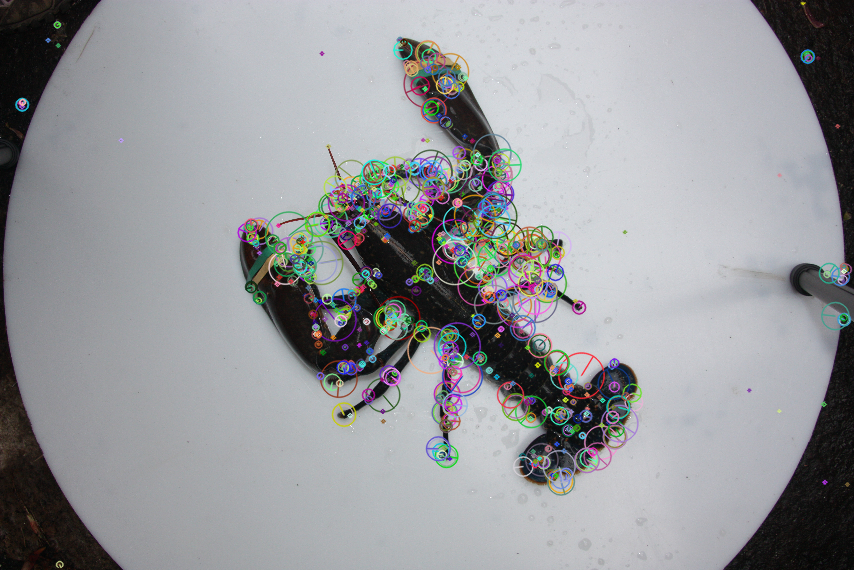
\includegraphics[width=\linewidth, keepaspectratio]{\imgpath/img-surf.png}
	\caption{SURF keypoint detection}
	\end{subfigure}
	
\caption{Comparison of different feature detection algorithms. The images have been scaled down after applying the detection to more clearly show the keypoints. Further comparison of the different detection algorithms on more images can be found in appendix \ref{apdx:cv-algos}}
\label{fig:kp-comparison}
\end{figure}
\begin{figure}[H]
%\centering
	\begin{subfigure}{0.45\textwidth}
	\includegraphics[width=\linewidth, keepaspectratio]{\imgpath/img-harris2.png}
	\caption{Harris corner detection}
	\end{subfigure}
	\hspace*{\fill}
	\begin{subfigure}{0.45\textwidth}
	\includegraphics[width=\linewidth, keepaspectratio]{\imgpath/img-shi-tomasi2.png}
	\caption{Shi-Tomasi corner detection}
	\end{subfigure}
	
	\vspace{0.5cm}
	
	\begin{subfigure}{0.45\textwidth}
	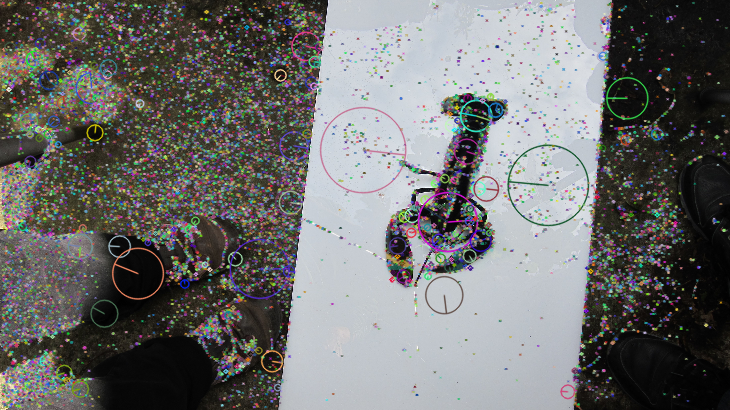
\includegraphics[width=\linewidth, keepaspectratio]{\imgpath/img-sift2.png}
	\caption{SIFT keypoint detection}
	\end{subfigure}
	\hspace*{\fill}
	\begin{subfigure}{0.45\textwidth}
	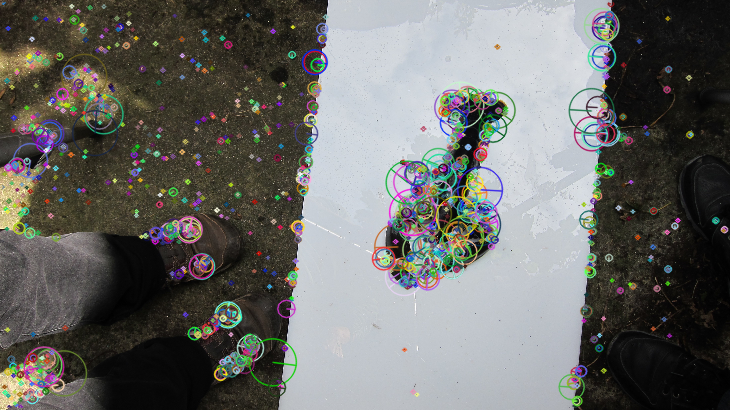
\includegraphics[width=\linewidth, keepaspectratio]{\imgpath/img-surf2.png}
	\caption{SURF keypoint detection}
	\end{subfigure}
	
\caption{Comparison of different feature detection algorithms on an image with more noise.}
\label{fig:kp-comparison-noise}
\end{figure}
\noindent
From visually seeing the effects of each algorithm, it can be seen that the corner detectors do not work very well for our purpose. This is to be expected, as they are meant to detect corners and not feature points. Although corner detectors have applications in image matching \cite{corner-detection}, our goal from feature detection is to be able to extract graph like objects or features to apply graph matching on and so corner detection is unsuitable as we are not looking to match the different images to each other directly and the comparisons in figure \ref{fig:kp-comparison-noise} and \ref{fig:kp-comparison} demonstrate why.

The keypoint detectors are able to provide better results for our objective, as we can see keypoints of important body parts being identified, such as the body, tail and claws. These keypoints are further able to be consistently identified from multiple images, showing that use of these algorithms are promising for automatically detecting the various parts of the lobster for construction of a graph. There is still a lot of irrelevant keypoints detected due to feature points in the backgrounds around the lobster, but we shall see later in section \ref{sec:kp-filter} that different methods can be applied to filter out unwanted keypoints. It is also non-trivial to create a graph from an outline of corners to represent the shape of a lobster, whereas the keypoints naturally translate well as nodes of a graph, with edges connecting them to form the shape and pose of a lobster. Because of these reasons, the keypoint detection algorithms in SIFT, SURF and ORB were further investigated while the corner detectors were discarded.

\begin{figure}[H]
\centering
TODO  fig of keypoint detector algorithm comparison
\caption{Comparison of different keypoint detection algorithms on multiple lobster images. See comparison of more images in appendix \ref{apdx:cv-algos}}
\end{figure}
\noindent

Between the different keypoint detection algorithms, SIFT was chosen as it gave the most consistent results and the kind of useful keypoints that are needed.


\subsection{Keypoint filtering}\label{sec:kp-filter}
From just running a SIFT detector on the lobster images, it can be seen that there are a lot of small keypoints that are unimportant for our purposes. There are also many keypoints around the lobster that we would like to filter out, as we want all our keypoints to be on the lobster. Initially, the classic vision approach for feature matching using the keypoint descriptors \cite{sift} was tried, but the results obtained were surprisingly poor. Because of this, a more novel approach was taken for filtering. The small keypoints are filtered out by specifying an octave where all keypoints coming from that octave or above are kept. Finally, remaining keypoints that are not on the lobster are filtered with a colour histogram method where the colour histograms of the keypoints are compared and any below a certain difference threshold are filtered away.

\subsubsection{SIFT descriptors}
In computer vision, keypoint descriptors obtained from detectors like SIFT and SURF are often used for feature matching \cite{cv-matching}. Lowe's paper \cite{sift} on the SIFT detector states that keypoints descriptors are highly distinctive, allowing a single feature to be correctly matching with good probability in a large database of features. This is exactly what we want, as we wish to extract the different features of a lobster (tail, claws, head). The only difference is we do not have a dataset of the lobsters, but not of dataset of individual lobster parts. 
\n
Because we do not have a dataset for individual parts, it made more sense to do the opposite of matching. Instead of using the distance between descriptors to match a detected keypoint with a known keypoint, the distance can be used as filter out keypoints that do not match closely to known ones. This distance can then be used as a threshold to filter more or less keypoints away. 
\n
As a test, the descriptor for the important body keypoint was taken from one image and calculated. The descriptor was then matched to the closest other keypoints on another image to see if the body could be identified again. 

\begin{figure}[H]
\centering
TODO keypoint descriptor matching other image
\caption{The image on the left shows the keypoint that the descriptor was calculated from and the image on the right is the closest TODO matched keypoints to that descriptor.}
\label{fig:kp-descriptor}
\end{figure}
\noindent
Figure \ref{fig:kp-descriptor} shows that the use of keypoint descriptors as a means of matching or filtering was not very reliable. TODO. As the traditional method of descriptors proved unreliable for our means, a slightly more novel method was needed to filter out keypoints.

\subsubsection{Octave filtering}
The method of filtering by the actual size of the keypoints was first looked at before looking at octaves. It was found to be less robust and less general than using octave levels. There are a few issues involved in using size of the keypoint for filter, namely how to choose a suitable threshold. The size threshold must be constant across all images, otherwise the method will not be able to generalise to unseen images. The size of the keypoints is directly related to the size of the original image, so any size filter threshold must be calculated based on the size of the image. This is not an issue, as a constant size threshold can be relative to the size of the image. However, with different sizes of lobsters, an aggressive threshold may remove important keypoints that we wanted to keep. Conversely a more conservative threshold would not remove enough keypoints and cause a large combinatorial explosion, a problem explained later in section \ref{sec:probabilistic-model} that we wish to avoid. This makes it difficult to set a good threshold as it would have to be arbitrarily defined and based solely on manual inspection of the images and keypoints sizes of the dataset. Furthermore, this seems to be quite a crude method with little support in existing research and doesn't take advantage of any properties in the SIFT algorithm. 

Octaves in SIFT are created by continually blurring an image. The idea behind this is to emulate looking at the image from different distances to get a varied set of keypoints. This means different features may be found at different octave levels. The high resolution of the images in our dataset causes many small keypoints to be found in the first few octave levels. These keypoints show many details that are irrelevant as we are concerned with the overall pose and size of the lobster.

\begin{figure}[H]
	\begin{subfigure}{0.5\textwidth}
	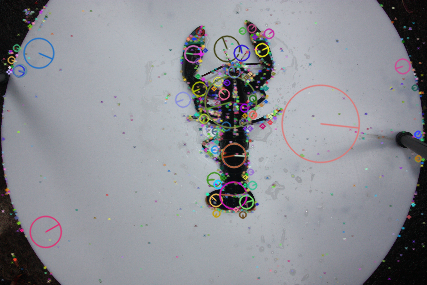
\includegraphics[width=\linewidth, keepaspectratio]{\imgpath/sift-raw.png}
	\caption{Before octave filtering}
	\end{subfigure}
	\hspace*{\fill}
	\begin{subfigure}{0.5\textwidth}
	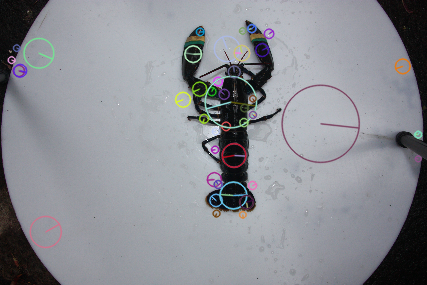
\includegraphics[width=\linewidth, keepaspectratio]{\imgpath/sift-octave.png}
	\caption{After octave filtering}
	\end{subfigure}
\caption{Before and after applying a filter on keypoints based on the octave level the keypoints were found in.}
\end{figure}
\noindent
From this observation, we can apply a filter on all keypoints found below a certain octave level so that we are only left with the larger keypoints that capture the features we are looking for. A filter for all keypoints found below octave level 3 was used. This octave level threshold is highly dependent on the size and resolution of the original image. An image with lower size and resolution may need a lower threshold or none at all as the lowered resolution effectively emulates octave levels applying their blur to the original image. 


\subsubsection{Colour histogram filtering}
After applying the octave filter, there still remains some irrelevant keypoints that need to be removed. Most notably are the keypoints found on the white background of the images. There have been studies \cite{color-histogram, color-filter} that show applying a colour filter to eliminate unwanted feature points can be quite effective, especially if the background is very different from the target of the image. Following from this, colour histograms of each keypoints were calculated and compared to a set of pre-defined histograms. The difference between the histograms was compared and only keypoints whose difference is above a certain threshold are kept. 

\begin{figure}[H]
	\begin{subfigure}{0.5\textwidth}
	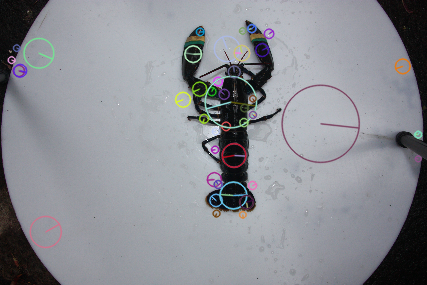
\includegraphics[width=\linewidth, keepaspectratio]{\imgpath/sift-octave.png}
	\caption{Octave filtering}
	\end{subfigure}
	\hspace*{\fill}
	\begin{subfigure}{0.5\textwidth}
	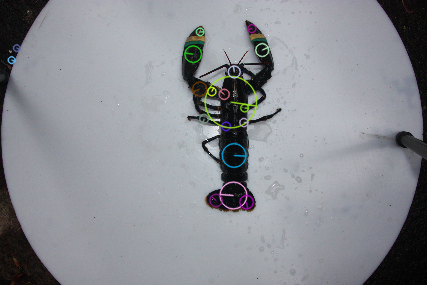
\includegraphics[width=\linewidth, keepaspectratio]{\imgpath/sift-histogram.png}
	\caption{Octave + colour histogram filtering}
	\end{subfigure}
\caption{Difference between applying only octave filtering and applying both octave and colour histogram filtering.}
\end{figure}
\noindent
The pre-defined histograms are taken from one of the lobster images from the dataset. A keypoint is taken and a mask applied to the image so only the area of the keypoint remains, then the histogram is calculated and saved as a NumPy array. The saved array can then be loaded later and compared to any keypoint to find the difference between them. Initially only one histogram was used, which was taken from the body keypoint of one image. However, this was not very effective as often the other keypoints had a large difference which meant the threshold had to be set to very low to capture important keypoints. This is not desirable as the lowered threshold causes more noisy keypoints to also be captured. To alleviate this issue, a separate histogram was calculated and saved for each different body part. This allowed TODO.
\begin{figure}[H]
\centering
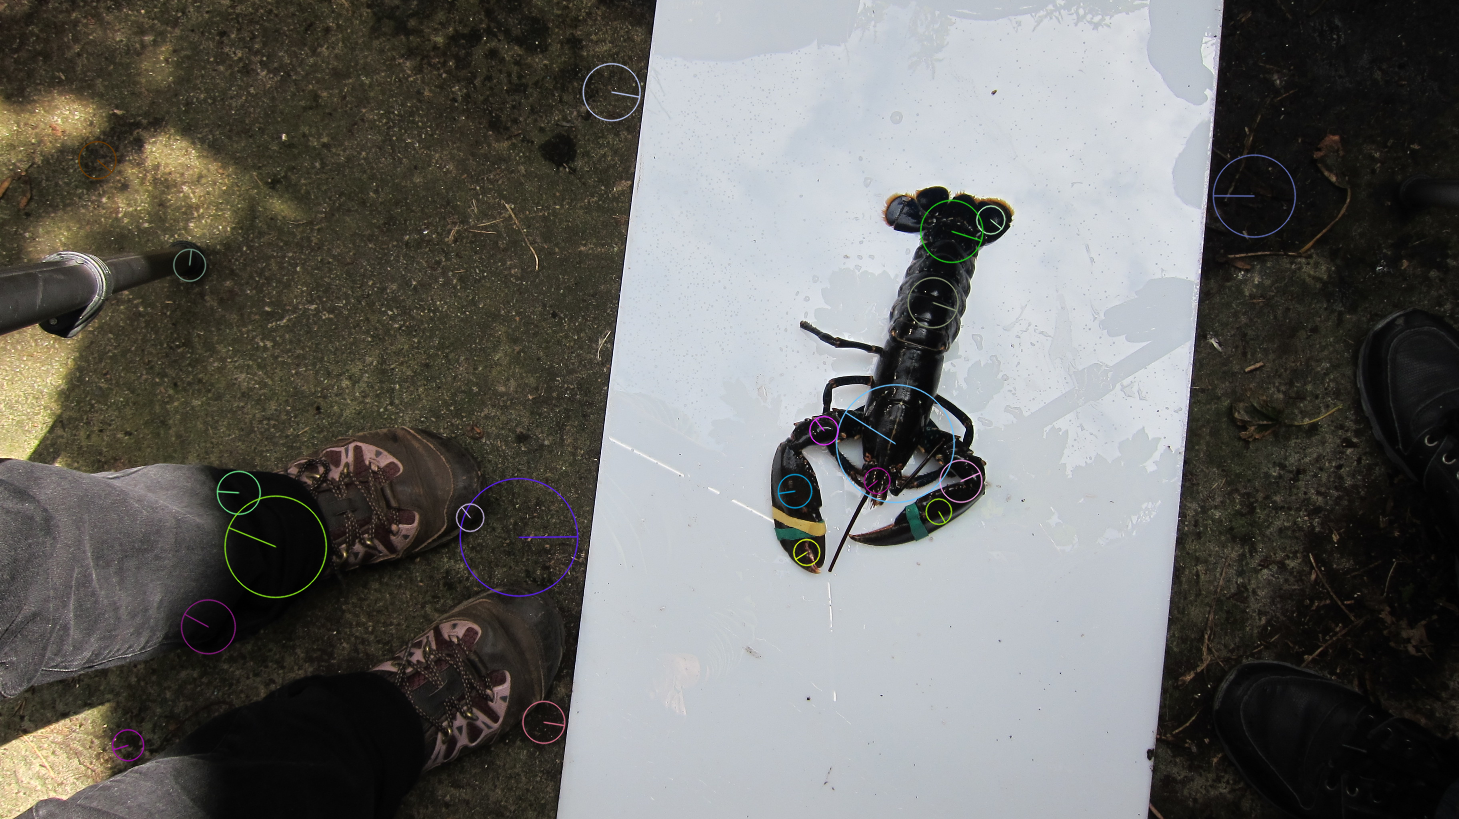
\includegraphics[width=1\textwidth, keepaspectratio]{\imgpath/noisy-keypoints.png}
\caption{Keypoints detected after filtering, showing the weakness of colour histogram filtering against noise.}
\label{fig:noisy-histogram}
\end{figure}
\noindent
A potential issue that was not fully explored is the application of this approach to noisy backgrounds. The colour histograms are effective due to the large contrast between the white background and the lobster. However, this means that keypoints detected in noisy backgrounds that have similar dark colours are not filtered out. Figure \ref{fig:noisy-histogram} shows an image with more in the background and it can be seen that multiple keypoints from the background not belonging to the lobster still are kept. The probabilistic models applied in the later stages help deal with this issue, as incorrect keypoints detected far away from the lobster will have low probabilities during graph matching and be filtered out. 

\subsection{Subgraph creation}
With a set of keypoints extracted and filtered from the image, the next step was to label the keypoints and create permutations of subgraphs to be matched. To reduce problems with combinatorial explosions when creating subgraph permutations, the number of labels assigned to each point and the size of the subgraphs have to be kept low. The idea of starting from creating subgraphs rather than try to create the entire lobster graph is to reduce the initial complexity of the problem. With a set of matched subgraphs, the larger lobster graph can be built incrementally. This method would also be more reliable than trying the whole lobster graph initially as more subgraphs can be taken into account during the rebuilding stage. Additionally, errors would be more easily accountable as the errors would only occur per mismatched subgraph rather than the whole lobster graph being mismatched in one step. 

\subsubsection{Node labelling}\label{sec:probabilistic-model}
A simple probabilistic model was used to determine how to label the keypoints through the use of Bayes' Theorem. For each keypoint, a probability is assigned for each label and a threshold applied to remove label probabilities that are too low.
\begin{equation}\label{eq:bayes-labelling}
P(\text{label}\ |\ \text{size}) = \frac{P(\text{size}\ |\ \text{label}) P(\text{label})} {P(\text{size})}
\end{equation}
The three probabilities $P(\text{size} | \text{label})$, $P(\text{label})$, $P(\text{size})$ are defined as follows:
\begin{itemize}
\item $P(\text{size} | \text{label})$ - This probability was found using a normal distribution for all sizes of the particular label found in the annotated dataset.
\item $P(\text{label})$ - This is defined as how often that label appears in the annotated dataset relative to the total number of all labels. For example, if there were a total of 100 labels and the \textit{body} label appears 20 times, then $P(\text{label} = \text{body}) = \frac{20}{100}$.
\item $P(\text{size})$ - The probability of keypoint sizes again uses a normal distribution for all keypoint sizes in the annotated dataset.
\end{itemize}
This method means multiple labels can be applied to the same keypoint and each separate labelling must be treated as a separate node during subgraph creation. The threshold for labelling represents the trade off between computation required and completeness. If the threshold is too high, then we may miss many potential labels. This is important because the size of the annotated dataset is quite small, so there is a high standard deviation in the distributions for label sizes. On the other hand, if the threshold is too low, then too many labels are applied, leading to a combinatorial explosion when creating the permutations of subgraphs. The result of the labelling process is a list of tuples containing a keypoint and its label. Having all the keypoints labelled, the next step is to create subgraphs where the nodes are represented by labelled keypoints and edges are defined  between the nodes to create the subgraph. 

\subsubsection{Subgraph permutations}
To create labelled subgraphs from the labelled keypoints, all possible permutations are produced. The size of the subgraph to create (and therefore the size of the permutation) is an important consideration in this step. The equation for the number of permutations of size $k$ from $n$ labelled keypoints is as follows:
\begin{equation}
P(n, k) = \frac{n!}{(n-k)!}
\end{equation}
A large $k$ would make the matching step easier as a larger subgraph conveys more information about the node labels and connectivity, so there would be fewer but more distinct matches. However, this would lead to considerably more permutations, for example, given 20 labelled nodes, there would be 6840 possible permutations for $k=3$ while $k=4$ would give 116280 permutations. Having this combinatorial explosion is unsustainable. Though a single permutation cannot contain the same keypoint with two different labels, each permutation of a single keypoint and its multiple labels must be explored. Further these are permutations so the order matters as it directly represents the connection of the nodes to edges.
\begin{figure}[H]
\centering
	\begin{subfigure}{0.45\textwidth}
	\centering
	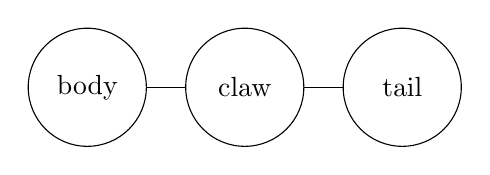
\begin{tikzpicture}
	\node (body) [circle, draw, minimum size=1.5cm] {body};
	\node (claw) [circle, draw, minimum size=1.5cm, right of=body, xshift=1cm] {claw};
	\node (tail) [circle, draw, minimum size=1.5cm, right of=claw, xshift=1cm] {tail};
	
	\draw (body) -- (claw);
	\draw (claw) -- (tail);
	\end{tikzpicture}
	\caption{Permutation (body, claw, tail)}
	\end{subfigure}
	\hspace*{\fill}
	\begin{subfigure}{0.45\textwidth}
	\centering
	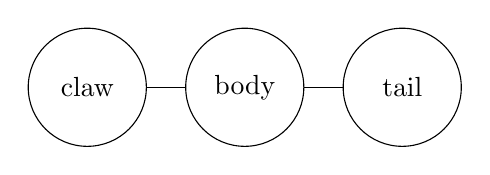
\begin{tikzpicture}
	\node (claw) [circle, draw, minimum size=1.5cm] {claw};
	\node (body) [circle, draw, minimum size=1.5cm, right of=claw, xshift=1cm] {body};
	\node (tail) [circle, draw, minimum size=1.5cm, right of=body, xshift=1cm] {tail};
	
	\draw (claw) -- (body);
	\draw (body) -- (tail);
	\end{tikzpicture}
	\caption{Permutation (claw, body, tail)}
	\end{subfigure}
\caption{The order of the permutations matters as it determines the edges between the nodes.}
\end{figure}
\noindent
A subgraph size of 3 was chosen in the end as it was a strong middle ground between retaining enough information for effective subgraph matching and not causing a large number of permutations to match. A size of 2 is ineffective for matching, it leads to too many successful matches because it is easy to find subgraphs of two nodes and one connecting edge as long as the labels are correct. However using 4 nodes as the subgraph led to too many permutations being produced, leading to a slow process in matching. This is why subgraphs of size 3 were chosen.



\subsection{Subgraph matching}
All subgraph permutations created are written as a query for GraphGrep to match. The reason for this matching step is to filter out subgraph configurations that are not  possible based on the annotated dataset. Any invalid configurations will not have appeared in the database of complete lobster graphs and therefore will not be matched. A single subgraph can match to multiple database graphs and can also match multiple times to a single database graph. This does not matter as extra matches are redundant information. 
\begin{figure}[H]
\centering
\begin{tikzpicture}
	\node (claw) [circle, draw, minimum size=1.5cm] {claw};
	\node (tail) [circle, draw, minimum size=1.5cm, right of=claw, xshift=1cm] {tail};
	\node (head) [circle, draw, minimum size=1.5cm, right of=body, xshift=1cm] {head};
	
	\draw (claw) -- (tail);
	\draw (tail) -- (head);
\end{tikzpicture}
\caption{An example of an invalid subgraph configuration that is filtered out by subgraph matching.}
\end{figure}

\begin{lstlisting}[caption={Example of matching output from GraphGrep}]
475:1:{(0,3),(1,1),(2,2)}
475:2:{(0,0),(1,3),(2,4)}
\end{lstlisting}

The output of running GraphGrep gives a list of graph ids of the subgraphs and database graphs that were matched. Any subgraph that appears in the list is taken as a matched permutation. After, there is a further step where the lengths of the edges between each node is taken into account. This acts as a late filter step for keypoints that may not be on the lobster, not allowing graph configurations where the points are too far apart to make sense. For example if the distance between an \textit{arm} node and \textit{claw} node is the same as the distance between a \textit{body} and \textit{tail}, the \textit{arm}/\textit{claw} permutation will be discarded. This is helpful in discarding keypoints that are far away from the lobster, for example on the edges of the background. Furthermore, this filters out subgraphs where the labelling was valid, but the distances between the nodes were not, which acts as a premature step to remove mislabelled subgraphs, for example if the tail or back was labelled as a claw and connected to a correctly labelled arm. 

\subsection{Graph building}\label{sec:graph-creation}
The final stage of the whole matching process is to take the pool of valid, matched and labelled subgraphs and piece together the complete lobster graph. Often there are many more subgraphs than are needed to rebuild the graph, so the best subgraphs and configurations should be chosen. To choose whether a subgraph was better than another, a na\"{i}ve Bayes probability model is used. The probability of each subgraph is calculated as the product of the probability of each node labelling and probability of each edge. 
\begin{equation}
P(\text{subgraph}) = \prod_{i=0}^n P(\text{node}_{i}) \cdot \prod_{j=0}^m P(\text{edge}_{j})
\end{equation}
where $n$ is the number of nodes and $m$ is the number of edges in the subgraph. The probability of each node labelling is already defined as it was used to assign the labels during the creation of the subgraph. It is the same as explained for equation \ref{eq:bayes-labelling}.
\begin{equation}
P(\text{node}) = P(\text{node.label}\ |\ \text{node.size})
\end{equation}
The probability of the edges is computed using Bayes' Theorem with a probability distribution for each type of edge based on the nodes it connects and its length. 
\begin{align}
\begin{split}
P(\text{edge}) &= P(\text{edge.length}\ |\ n_{1} \wedge n_{2}) \\
 &= \frac{P(n_{1} \wedge n_{2}\ |\ \text{edge.length}) \cdot P(\text{edge.length})}{P(n_{1}) \cdot P(n_{2})}
\end{split}
\end{align}
Each type of edge is uniquely defined by the two nodes it connects and so the probability of the edge takes that into account. To prevent floating point issues during implementation, the sum of logs is used rather than the product of the probabilities. 
\n
As stated before, a single keypoint can also be contained in multiple subgraphs. These cases have to be treated carefully as it is valid for those more than one of those multiple subgraphs to appear in the final lobster graph. An easy example of this is a body keypoint which has multiple subgraphs. One subgraph could contain the tail and back while another contains the arm and claw. In this case they are both valid because they could both be part of the final graph. Because of this, subgraphs in the pool cannot be discarded simply because they contain the same keypoint and label as another. Further, it is inevitable that multiple subgraphs with the same keypoint are used to be able to build a graph that is fully connected, otherwise additional rules will be need to define how two subgraphs should be connected.
\n
With these considerations in mind, three different methods were used to build up the lobster graph from subgraphs, one of which gave poor results and was not used in the final evaluation. 
\begin{figure}[H]
\centering
	\begin{subfigure}{0.32\textwidth}
	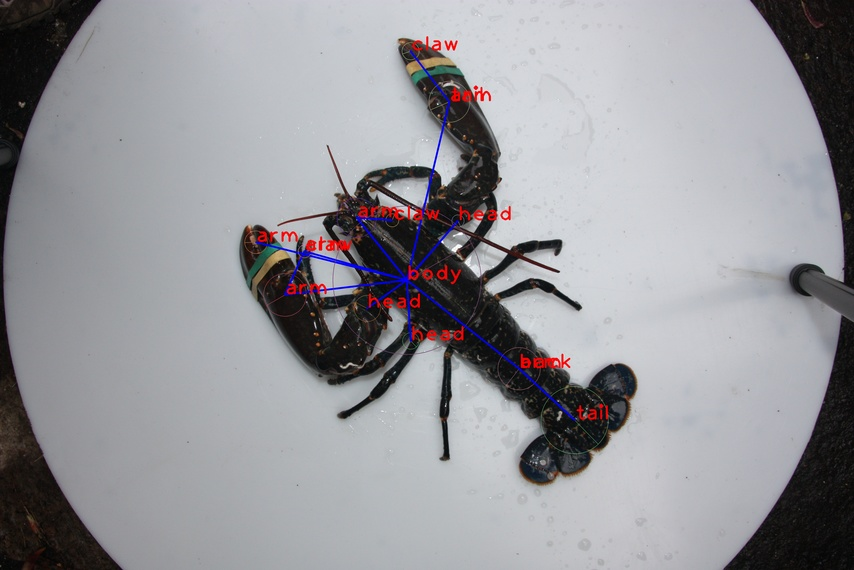
\includegraphics[width=\textwidth, keepaspectratio]{\imgpath/kp-method.JPG}
	\caption{Keypoint method}	
	\end{subfigure}
	\hspace*{\fill}
	\begin{subfigure}{0.32\textwidth}
	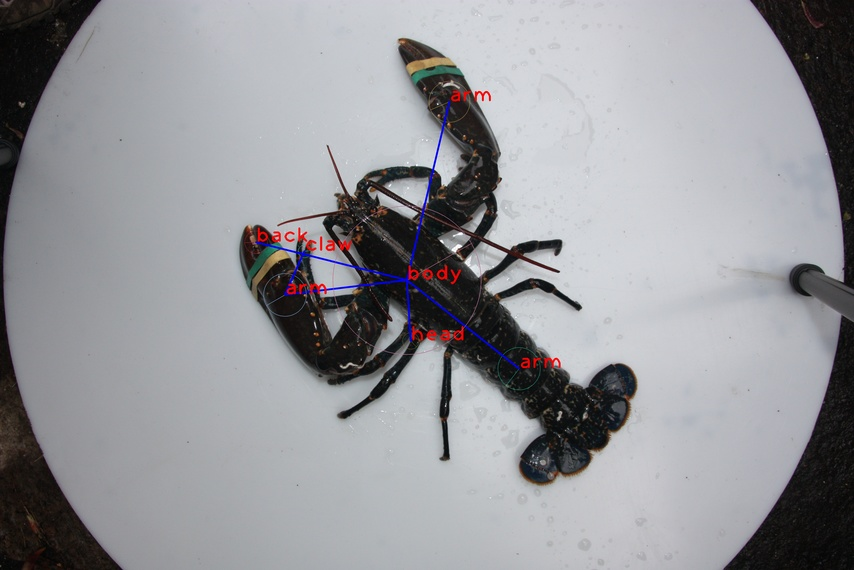
\includegraphics[width=\textwidth, keepaspectratio]{\imgpath/label-method.JPG}
	\caption{Label method}
	\end{subfigure}
	\hspace*{\fill}
	\begin{subfigure}{0.32\textwidth}
	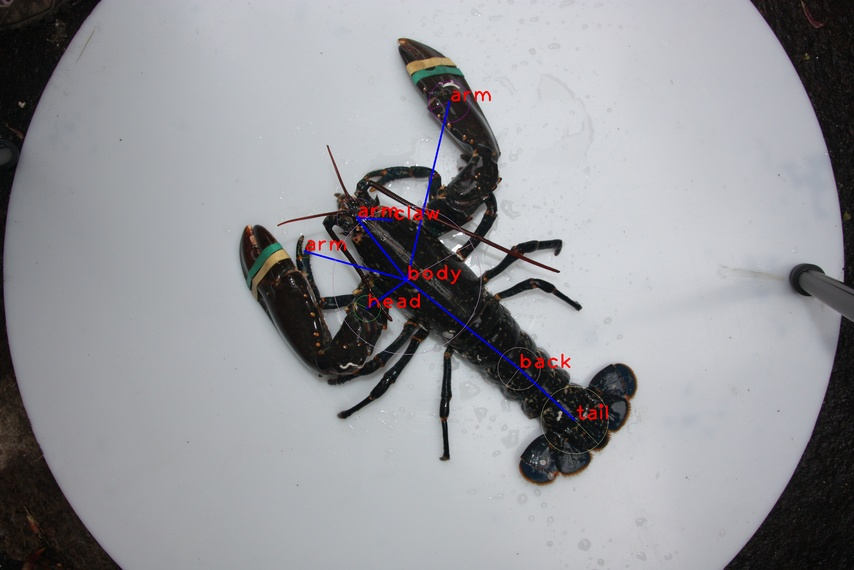
\includegraphics[width=\textwidth, keepaspectratio]{\imgpath/graph-method.JPG}
	\caption{Graph method}
	\end{subfigure}
\caption{Comparison of the three different methods for rebuilding the complete lobster graph from matched subgraphs.}
\end{figure}
\noindent
The three different methods are as follows:
\begin{enumerate}
\item \textbf{Keypoint method} - The initial method explored was to ensure every keypoint is used when rebuilding the subgraph. This will make sure that no keypoints are missed. For every keypoint that was detected and not filtered away, the subgraph with the highest combined probability is chosen. Some chosen subgraphs are removed to prevent overlaps where the same keypoint is given multiple labels. This removal is again based on probability where the subgraph with the highest probability is kept. The main issue with this method is it is very reliant on good keypoint detection and filtration. Any incorrectly detected keypoints will be included this process which leads to errors of labelling many irrelevant points. As such, more sophisticated methods were explored that do not rely so heavily on the keypoints detected.
\item \textbf{Label method} - In this method, a list of canonical required labels is used to choose the subgraphs for the final lobster graph. This ensures that the complete set of labels needed for the complete lobster is used and found where possible and very few additional labels past the canonical ones will be included. To build the complete graph, the most probable subgraph is chosen for each label in the canonical list of labels. Then, overlap is checked by comparing the keypoints and labels in each subgraph. This is done to make sure no keypoint has two different labels but will allow one keypoint to be contained in multiple subgraphs. Further, when a probably subgraph is chosen, the labels it contains are removed from the canonical list. The final output is the set of most probable subgraphs that contain as many of the canonical labels as possible without repetition. 
\item \textbf{Graph method} - The final method explored takes into account graph properties of how nodes are connected rather than just choosing based on canonical labels. The weakness of the label method is not taking into account any relations between the nodes. Here, a canonical \textit{graph} is defined which specifies both the labels and the connections between them. For each edge in the graph, matched subgraphs are chosen based on whether they contain the same node connections as the canonical edge. Again the same method of choosing the subgraph with the highest probability and removing overlaps was used to prevent duplicate labelling.
\end{enumerate}
\noindent
In section \ref{sec:results}, the results of using both the labelling and graph methods are compared and analysed to see how well they work.


